\section{Spielbeschreibung}

\begin{frame}
	\frametitle{Tisch und Spielelemente}
	\begin{figure}
		\centering
		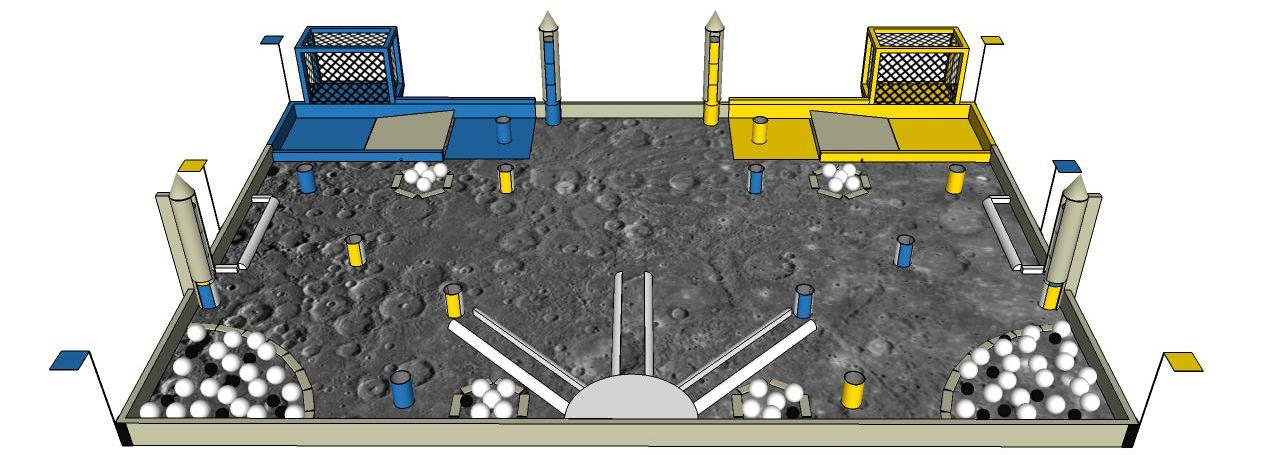
\includegraphics[width = 13cm]{../images/presentation/spielfeldElemente.jpg}
	\end{figure}
	
\end{frame}

\begin{frame}
	\frametitle{Aufgaben und Punkte}
	
	\begin{figure}[H]
		\centering
		\begin{tabular}{|c|c|}
			\hline
			Ressourcen im Startfeld & 2 Punkte\\
			\hline
			\textit{Titanium Ores} in \textit{Cargo Bay} & 3 Punkte\\
			\hline
			\textit{Lunar Modules} in \textit{Moonbase} & 10 Punkte\\
			\hline
			\textit{Funny Action} & 20 Punkte\\
			\hline
			Bonus für aus dem Startfeld fahren & 15 Punkte\\ 
			\hline
			\hline
			\textit{Moon Rocks} & 0 Punkte\\
			\hline
			Strafe für unfaires und regelwidriges Verhalten & -20 Punkte\\
			\hline
		\end{tabular}	
	\end{figure}
\end{frame}

\begin{frame}
	
	%todo: Nicht benötigt!!
	
	\frametitle{Anforderungen an die Roboter}
	
	\begin{itemize}
		\item mechanische Abmessungen gemäss Reglement
		\item Roboter bewegen sich autonom
		\item keine Kollisionen mit Gegner
		\item keine gefährliche Techniken und Materialien (Pyrotechnik, starke Laser, ...)
	\end{itemize}
	
\end{frame}

\begin{frame}
	
	%todo Nicht benötigt
	
	\frametitle{Wettbewerb}
	
	\begin{itemize}
		\item Homologation
	\end{itemize}
	\begin{itemize}
		\item 3 min Vorbereitungszeit
		\item 90 s Spiel
		\item \textit{Funny Action}
	\end{itemize}
	\begin{itemize}
		\item Finale \textit{Best-of-three}
	\end{itemize}
\end{frame}